\begin{figure}[tbp]
\begin{center}
\includegraphics[width=0.48\textwidth]{figure/sn_z1_z2.eps}
\end{center}
\vspace{-0.7cm}
\caption{Cumulative S/N, assuming Planck noise at 217 GHz, $f_{sky}=0.8$. 
}
\label{fig:sn}
\end{figure}
%In real surveys, when we calculate the cross angular power spectrum $C_l$ between reconstructed kSZ signals and CMB measurements, we will have to face statistical errors. 
%They can be approximated as:
Taking into account primary CMB and facility noises, 
the chance to seperate kSZ signal from statistical errors could be estimated 
as:
%\begin{eqnarray}
 %   \frac{\Delta C_l}{C_l}\simeq \frac{1}{r\sqrt{(2l+1)\Delta l f_{sky}}}\sqrt{\frac{C_l^{\mr{CMB}}+C_l^{kSZ}+C_l^{\mr{CMB},N}}{C_l^{kSZ,\Delta z}}(1+\frac{C^N_{\hat \Theta}}{C_{\hat \Theta}})}\,
%\end{eqnarray}
\begin{eqnarray}
    \frac{S}{N}&=&\frac{C_l}{\Delta C_l}\\\nonumber
               &\simeq&
    r\sqrt{(2\ell+1)\Delta l f_\mathrm{sky}}\sqrt{\frac{C_l^{\mathrm{kSZ},\Delta z}}{C_l^{\mr{CMB}}+C_l^\mathrm{kSZ}+C_l^{\mr{CMB},N}}}
\end{eqnarray}
Where $C_l^\mathrm{CMB}$ is the angular powerspectrum of primary CMB 
;
$C_l^\mathrm{CMB,N}$ indicates the facility noises; 
$C_l^{\mathrm{kSZ},\Delta z}$ is the kSZ signal from a certain redshift bin; 
r is the correlation coefficients we get; 
$f_\mathrm{sky}$ is the percent of sky area covered by both surveys.

In our case, $C_l^\mr{CMB}$ is calculated from CAMB \cite{CAMB}. 
$C_l^\mr{CMB,N}$ is estimated with Planck results \cite{Planck2015} at 217GHz.
$C_l^\mathrm{CMB,N}=(\sigma_{p,T}\theta_\mathrm{FWHM})^2W_l^{-2}$;  
where $\sigma_{p,T}=8.7\mu K_\mathrm{CMB}$ is Sensitivity per beam solid angle, 
$\theta_\mathrm{FWHM}\sim 5'$ is the effective beam FWHM, 
$W_l=\exp[-\ell(\ell+1)/2\ell^2_\mathrm{beam}]$ is the smoothing window function, 
with $\ell _\mathrm{beam}=\sqrt{8\ln2}/\theta_\mathrm{FWHM}$. 
We choose $f_\mathrm{sky}=0.8$ according to claimed 21 cm intensity mapping survey area. 
$C_l^{\mathrm{kSZ},\Delta z}$ is calculated within two bins of size 1200 Mpc/h, centered at redshift 1,2 respectively.

The cumulative S/N is demonstrated in Fig.\ref{fig:sn}. 
The low correlation in $z=2$ is compensated by the high electron density 
and the overall S/N could well reach 50 with HIRAX.

With noise level of Planck, 
the resolution of HIRAX already cover most important $\ell$s. 
However, with $4_\mathrm{th}$ generation facilities, 
more detectable modes will apprear in higher $\ell$s, 
and better S/N could be expected with longer baselines like SKA.

